% -----------------------------------------------------------------------------
% Master thesis in the study program computational mechanics
%
% B.Sc. Rezha Adrian Tanuharja - 03751261
% M.Sc. Felix Schneider (supervisor)
%
% chapters/discussion/surrogate/point_A.tex
% Last edited 03 November 2023
% -----------------------------------------------------------------------------

\subsection{Vertical Acceleration at Node A}
\label{ssec: surrogate point A}

Figure \ref{FRF_rRPCE_A_A_2} shows the medians and the interquartile ranges of relative empirical errors of FRF approximations for the regular RPCE models at $\omega=9.0$ rad/s.
The figure displays error values at various sizes of the training data, relative to the total number of bases in the models.
\begin{figure}[H]
    \centering
    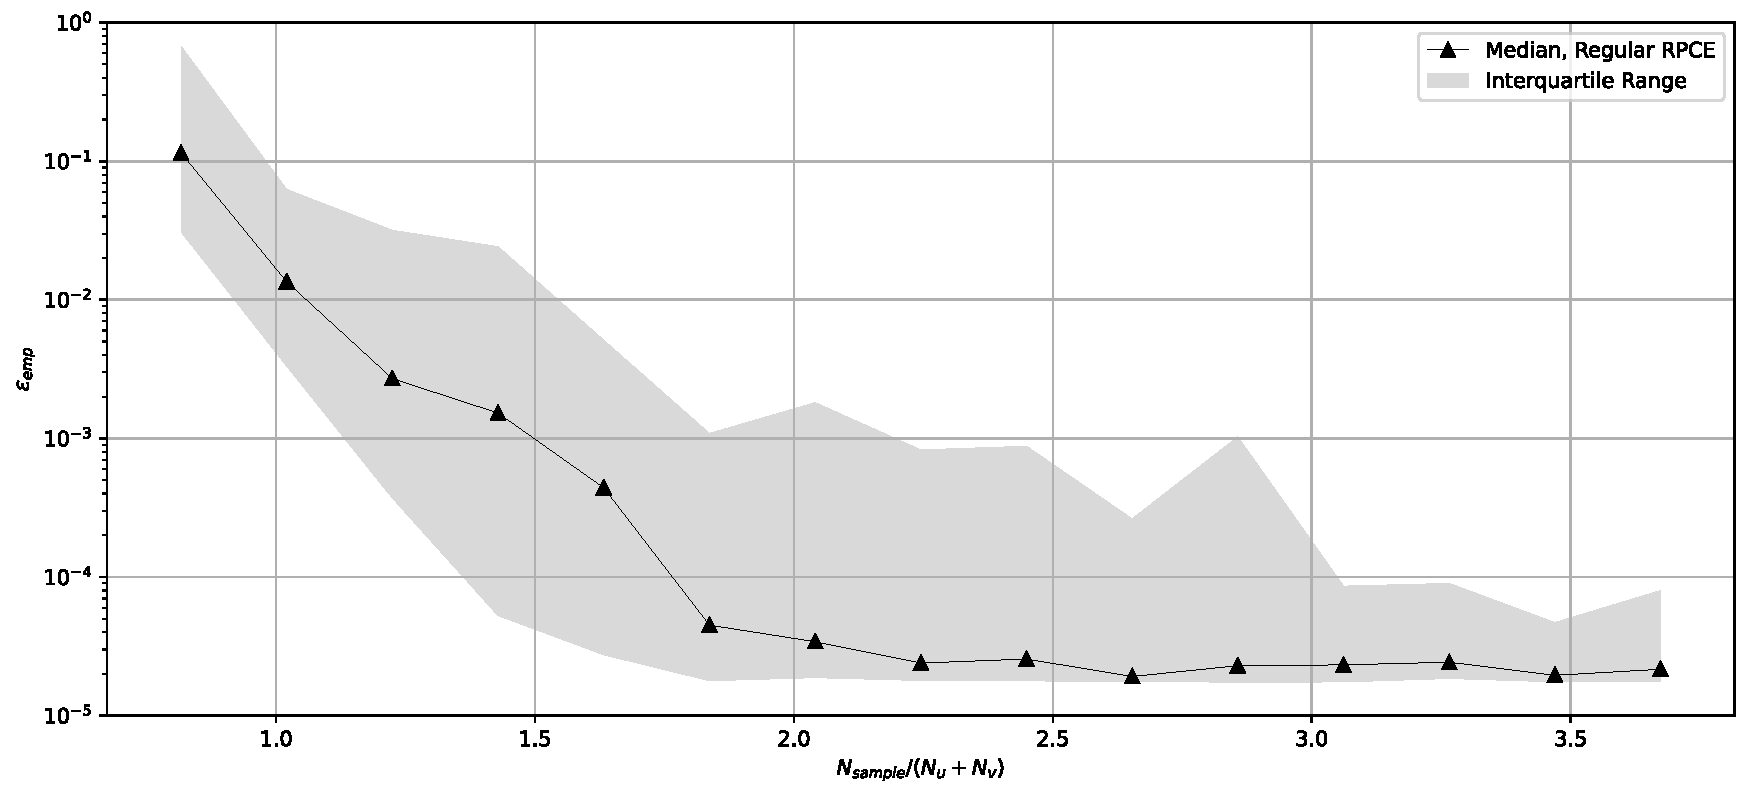
\includegraphics[width=1.0\textwidth]{
        plots/surrogate/plot_1P_A_2.pdf
    }
    \caption{%
        Relative Empirical Errors of $H_{AA}$ for Regular RPCE Models at $\omega=9.0$ rad/s
    }
    \label{FRF_rRPCE_A_A_2}
\end{figure}
The figure above shows that the relative empirical error decreases as the size of training data increases.
The medians converge when the size of the training data is approximately $2.0$ to $2.5$ times the total number of bases in the models.

Figure \ref{FRF_sRPCE_A_A_2} shows the medians and the interquartile ranges of relative empirical errors of the FRF approximations for the regular and sparse RPCE models at $\omega=9.0$ rad/s.
\begin{figure}[H]
    \centering
    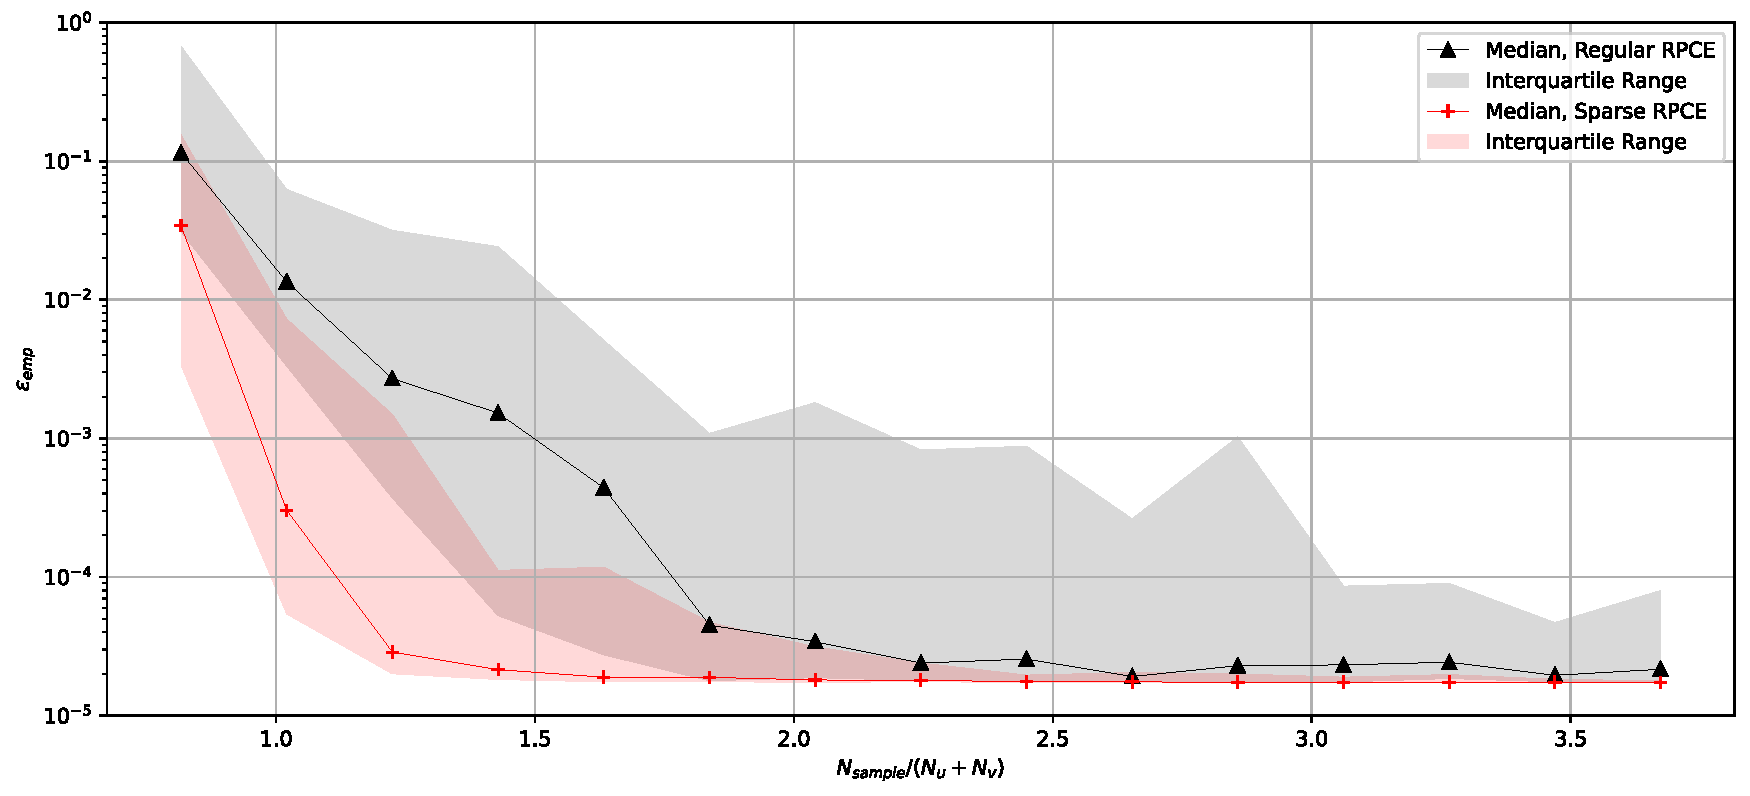
\includegraphics[width=1.0\textwidth]{
        plots/surrogate/plot_1_A_2.pdf
    }
    \caption{%
        Relative Empirical Errors of $H_{AA}$ for Regular and Sparse RPCE Models at $\omega=9.0$ rad/s
    }
    \label{FRF_sRPCE_A_A_2}
\end{figure}
Overall, the sparse RPCE models have lower relative empirical errors when training data sizes are small.
The medians converge when the size of the training data is approximately $1.5$ to $2.0$ times the total number of bases in the models.

Figures \ref{FRF_sRPCE_A_A_3} to \ref{FRF_sRPCE_A_A_6} show the relative empirical errors for the regular and sparse RPCE models at various frequencies.
\begin{figure}[H]
    \centering
    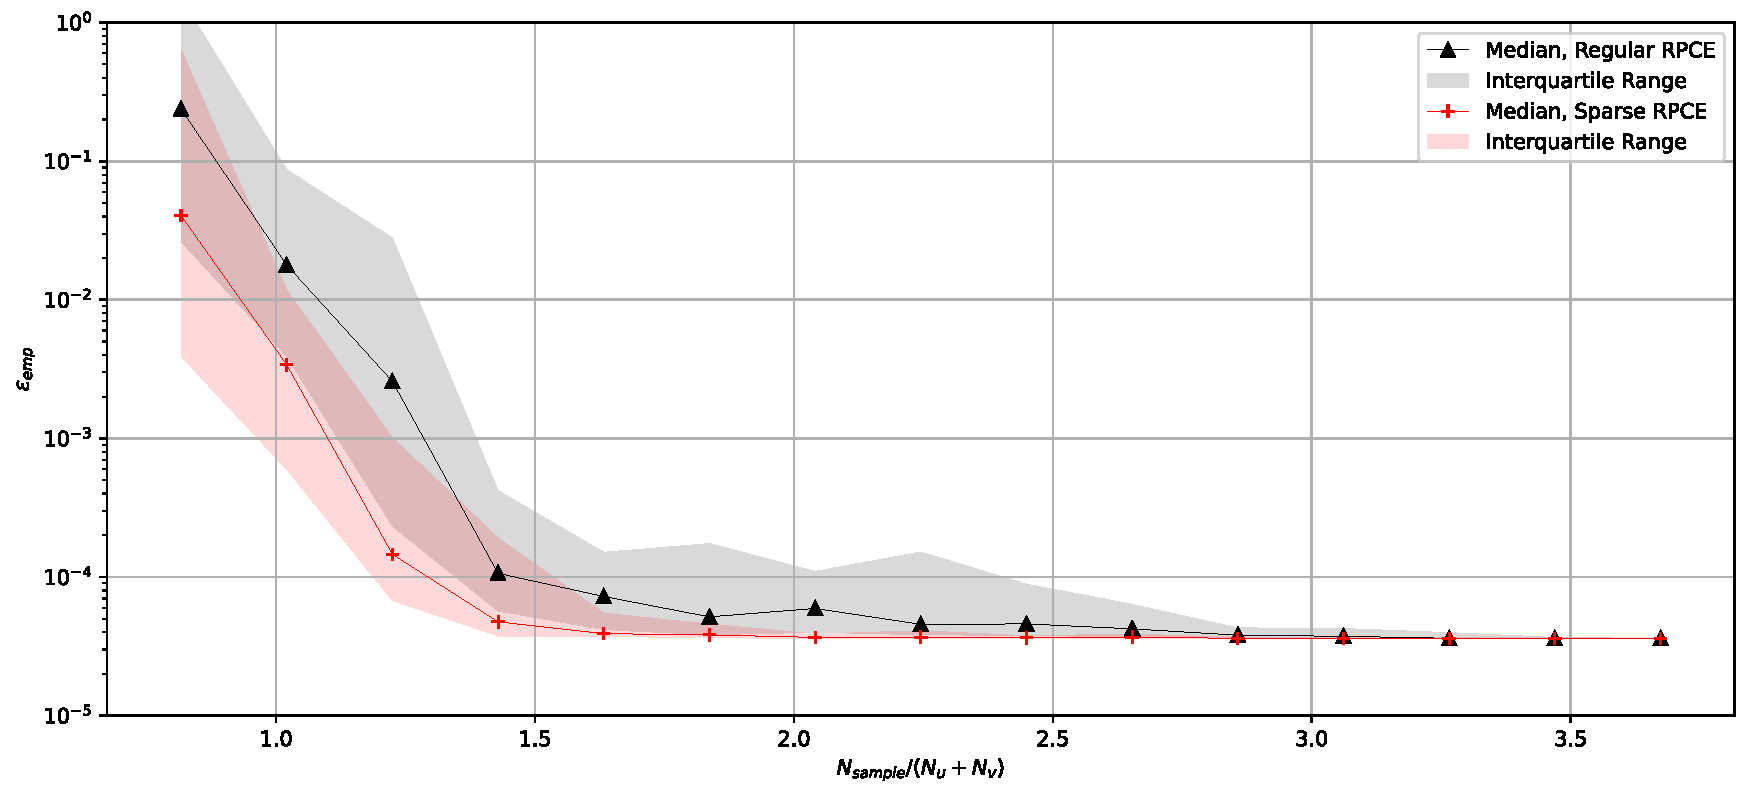
\includegraphics[width=1.0\textwidth]{
        plots/surrogate/plot_1_A_3.pdf
    }
    \caption{%
        Relative Empirical Errors of $H_{AA}$ for Regular and Sparse RPCE Models at $\omega=9.5$ rad/s
    }
    \label{FRF_sRPCE_A_A_3}
\end{figure}
\begin{figure}[H]
    \centering
    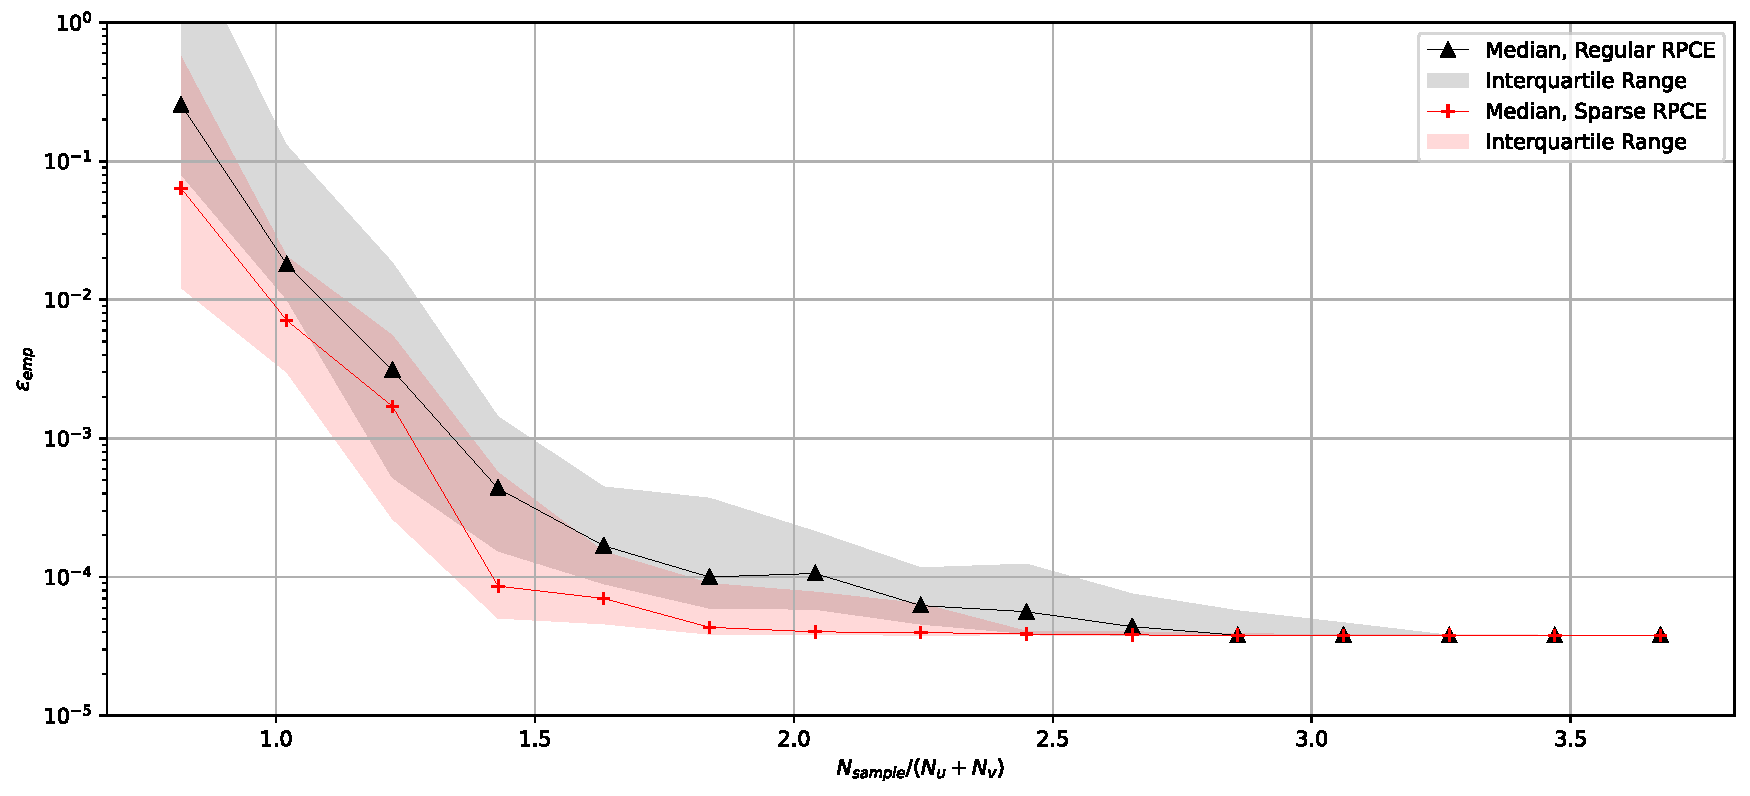
\includegraphics[width=0.85\textwidth]{
        plots/surrogate/plot_1_A_4.pdf
    }
    \caption{%
        Relative Empirical Errors of $H_{AA}$ for Regular and Sparse RPCE Models at $\omega=10.0$ rad/s
    }
    \label{FRF_sRPCE_A_A_4}
\end{figure}
\begin{figure}[H]
    \centering
    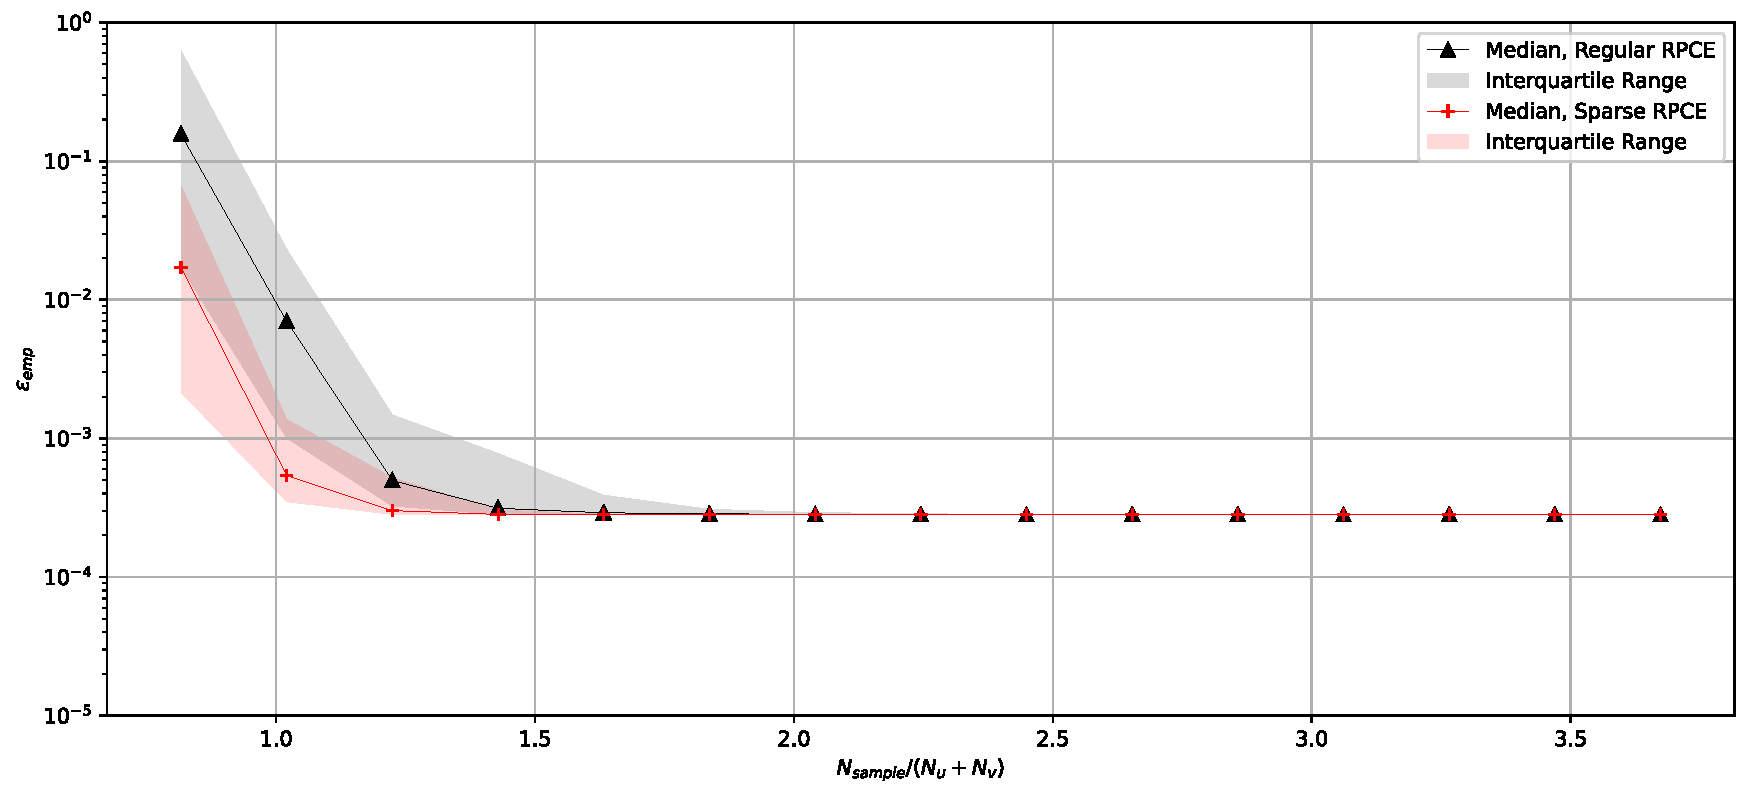
\includegraphics[width=0.85\textwidth]{
        plots/surrogate/plot_1_A_5.pdf
    }
    \caption{%
        Relative Empirical Errors of $H_{AA}$ for Regular and Sparse RPCE Models at $\omega=10.5$ rad/s
    }
    \label{FRF_sRPCE_A_A_5}
\end{figure}
\begin{figure}[H]
    \centering
    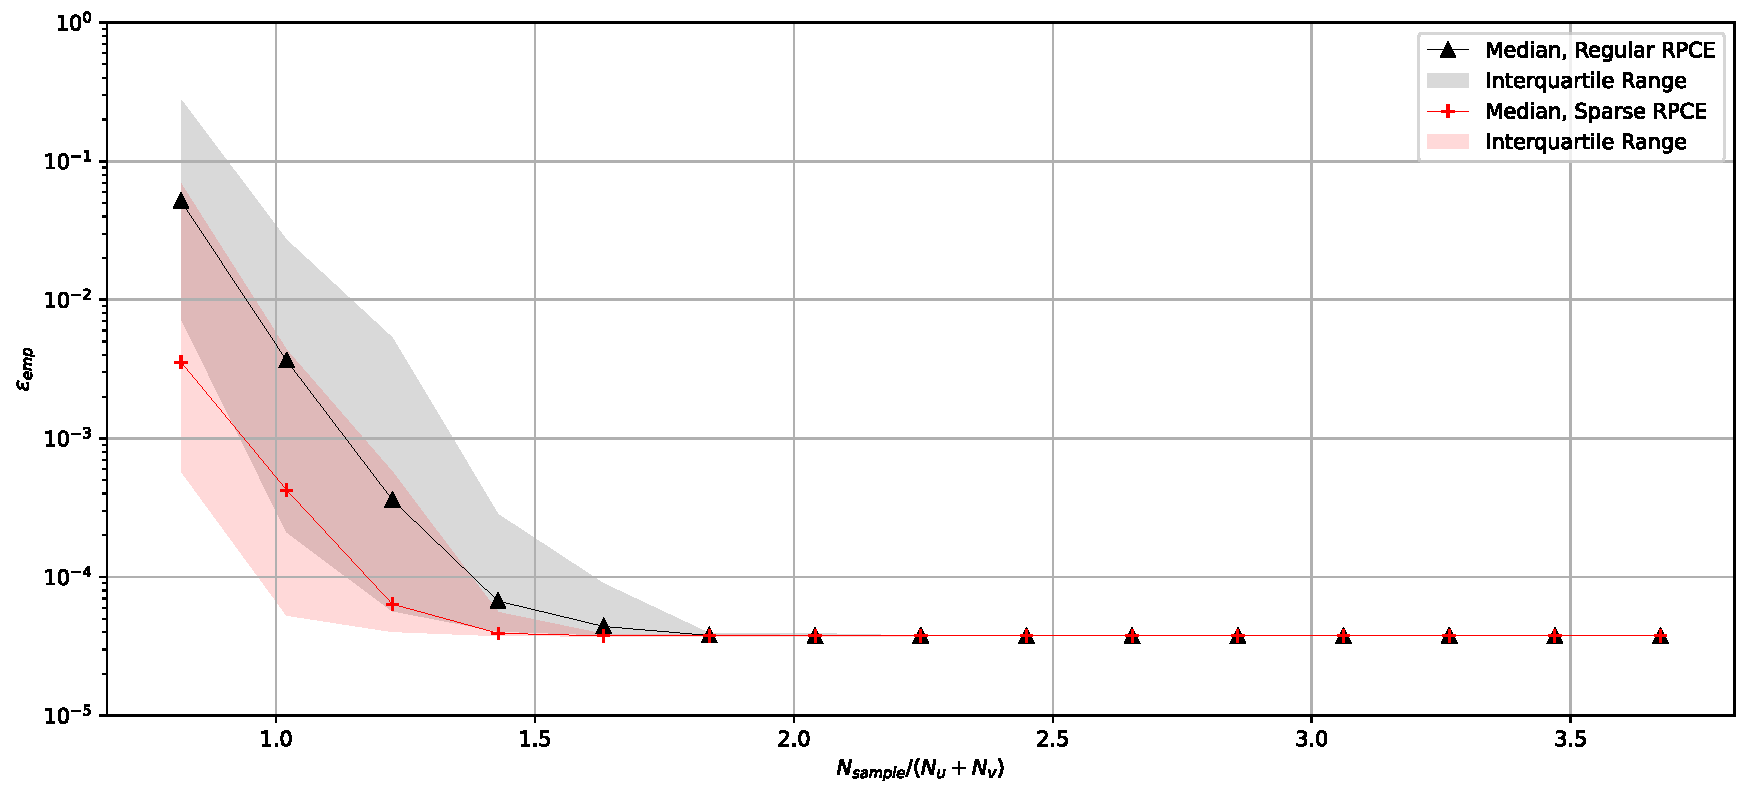
\includegraphics[width=0.85\textwidth]{
        plots/surrogate/plot_1_A_6.pdf
    }
    \caption{%
        Relative Empirical Errors of $H_{AA}$ for Regular and Sparse RPCE Models at $\omega=11.0$ rad/s
    }
    \label{FRF_sRPCE_A_A_6}
\end{figure}
The figures above exhibit similar trends: the sparse RPCE models have lower relative empirical errors when training data sizes are small.
% The relative empirical errors for the regular and sparse RPCE models at other frequencies are available in the appendix.

To dive deeper into the differences between the regular and sparse RPCE models, the author evaluates the relative mean and variance errors.
Figures \ref{mean_rRPCE_A_A_2} and \ref{var_rRPCE_A_A_2} show the medians and interquartile ranges of relative mean errors and the relative variance errors for regular RPCE models at $\omega=9.0$ rad/s.
\begin{figure}[H]
    \centering
    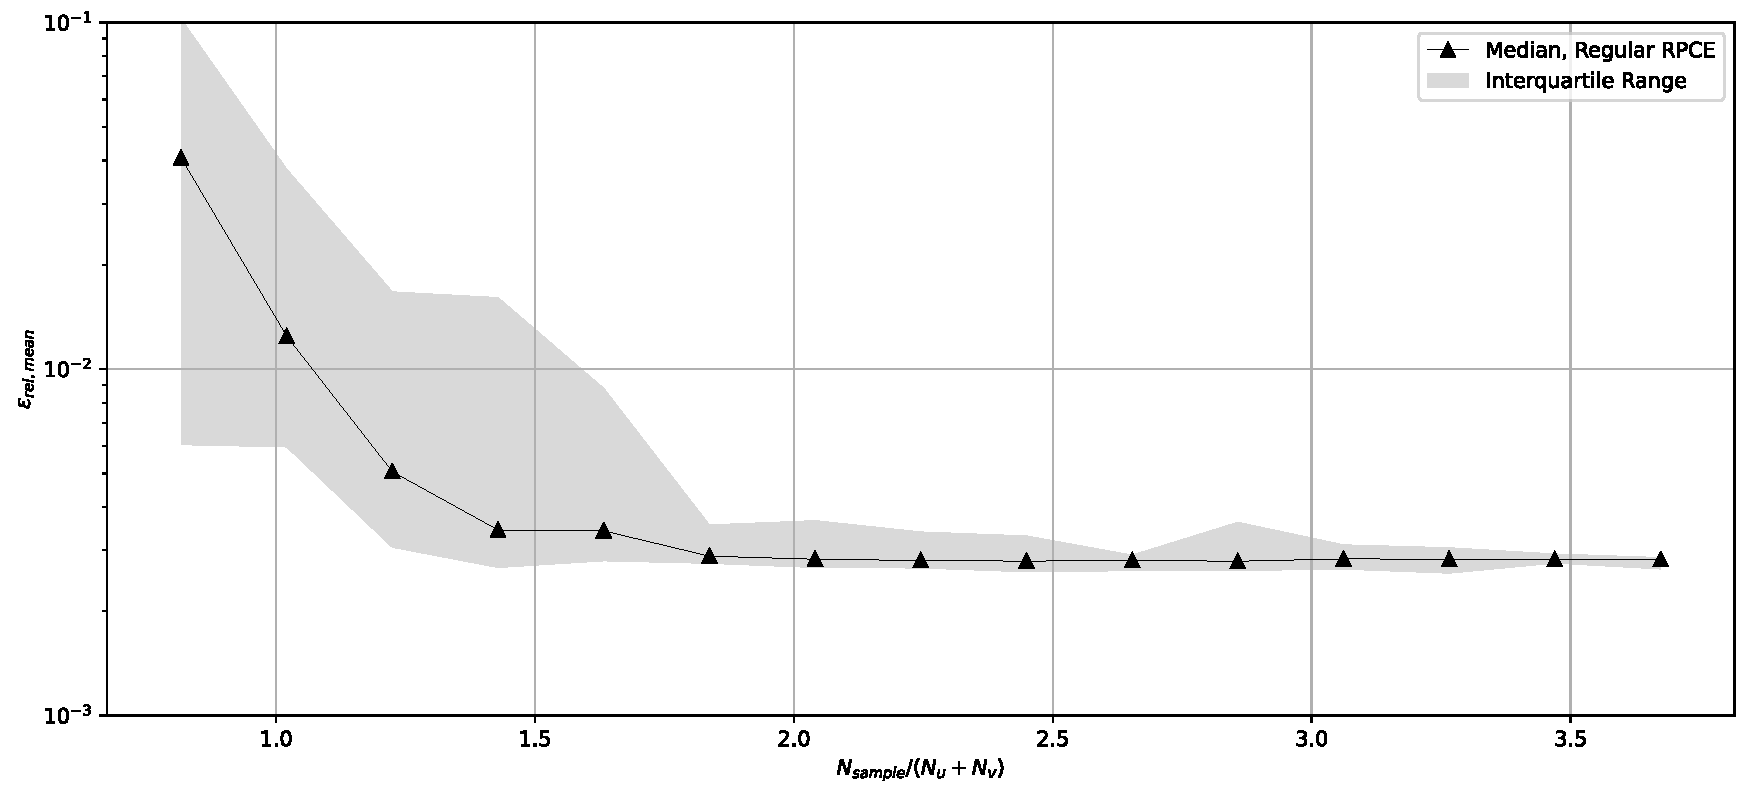
\includegraphics[width=1.0\textwidth]{
        plots/surrogate/plot_2P_A_2.pdf
    }
    \caption{%
        Relative Mean Errors of $\left|H_{AA}\right|$ for Regular RPCE Models at $\omega=9.0$ rad/s
    }
    \label{mean_rRPCE_A_A_2}
\end{figure}
\begin{figure}[H]
    \centering
    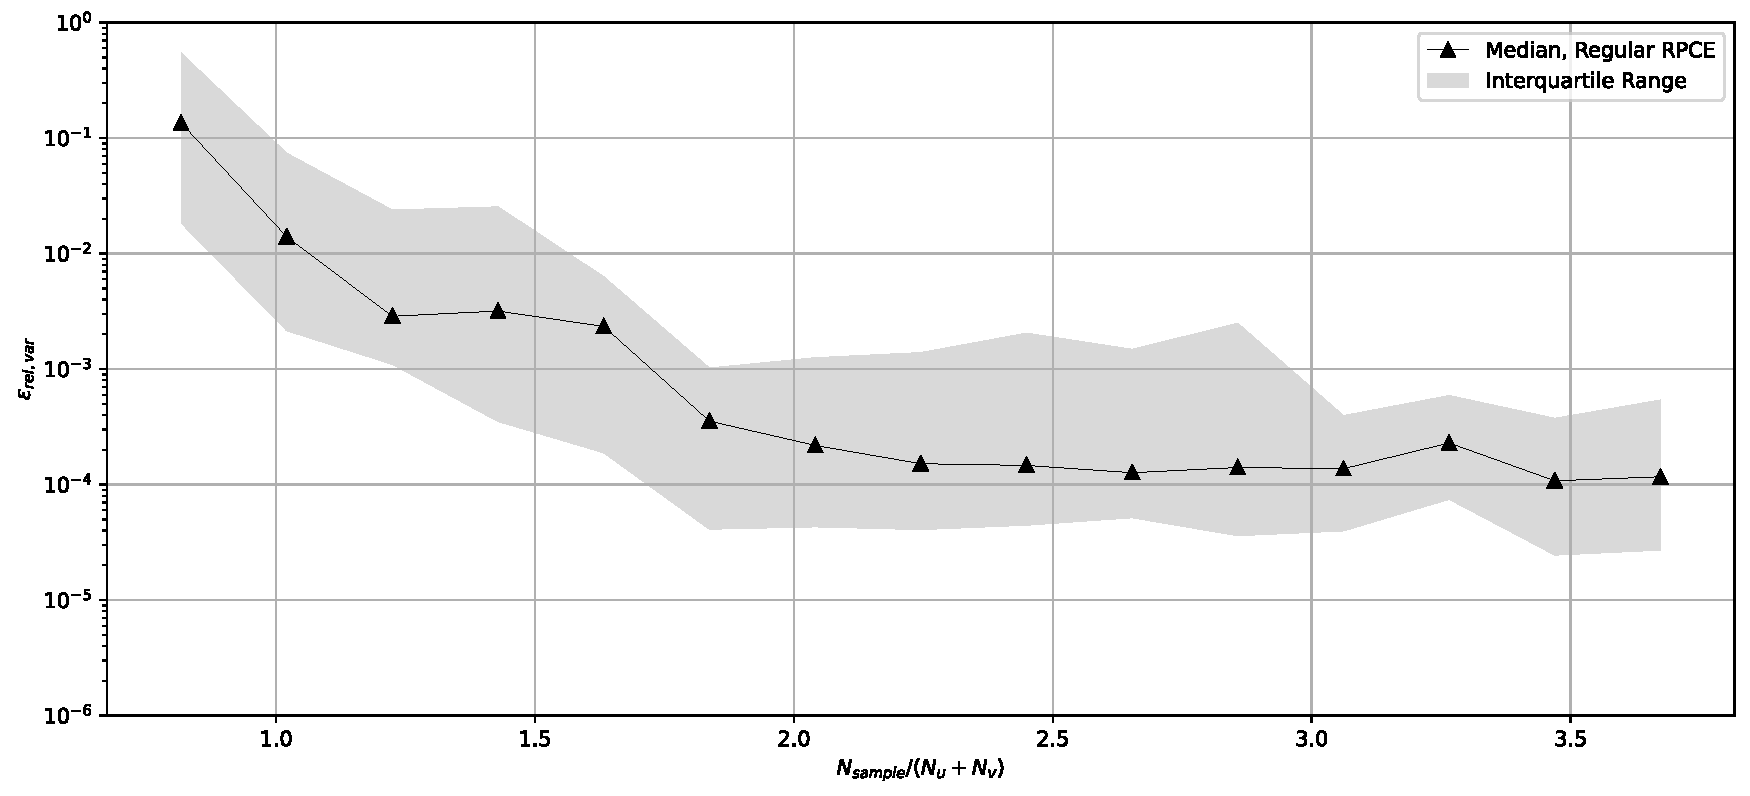
\includegraphics[width=1.0\textwidth]{
        plots/surrogate/plot_3P_A_2.pdf
    }
    \caption{%
        Relative Variance Errors of $H_{AA}$ for Regular RPCE Models at $\omega=9.0$ rad/s
    }
    \label{var_rRPCE_A_A_2}
\end{figure}
Similar to the relative empirical errors, the medians converge when the size of training data is approximately $2.0$ to $2.5$ times the number of bases in the RPCE models.
Subsequently, the author compares the relative mean errors and the relative variance errors from regular RPCE models with those from sparse RPCE models.
Figure \ref{mean_sRPCE_A_A_2} shows the medians and interquartile ranges of relative mean errors of the FRF approximations for regular and sparse RPCE models at $\omega=9.0$ rad/s.
\begin{figure}[H]
    \centering
    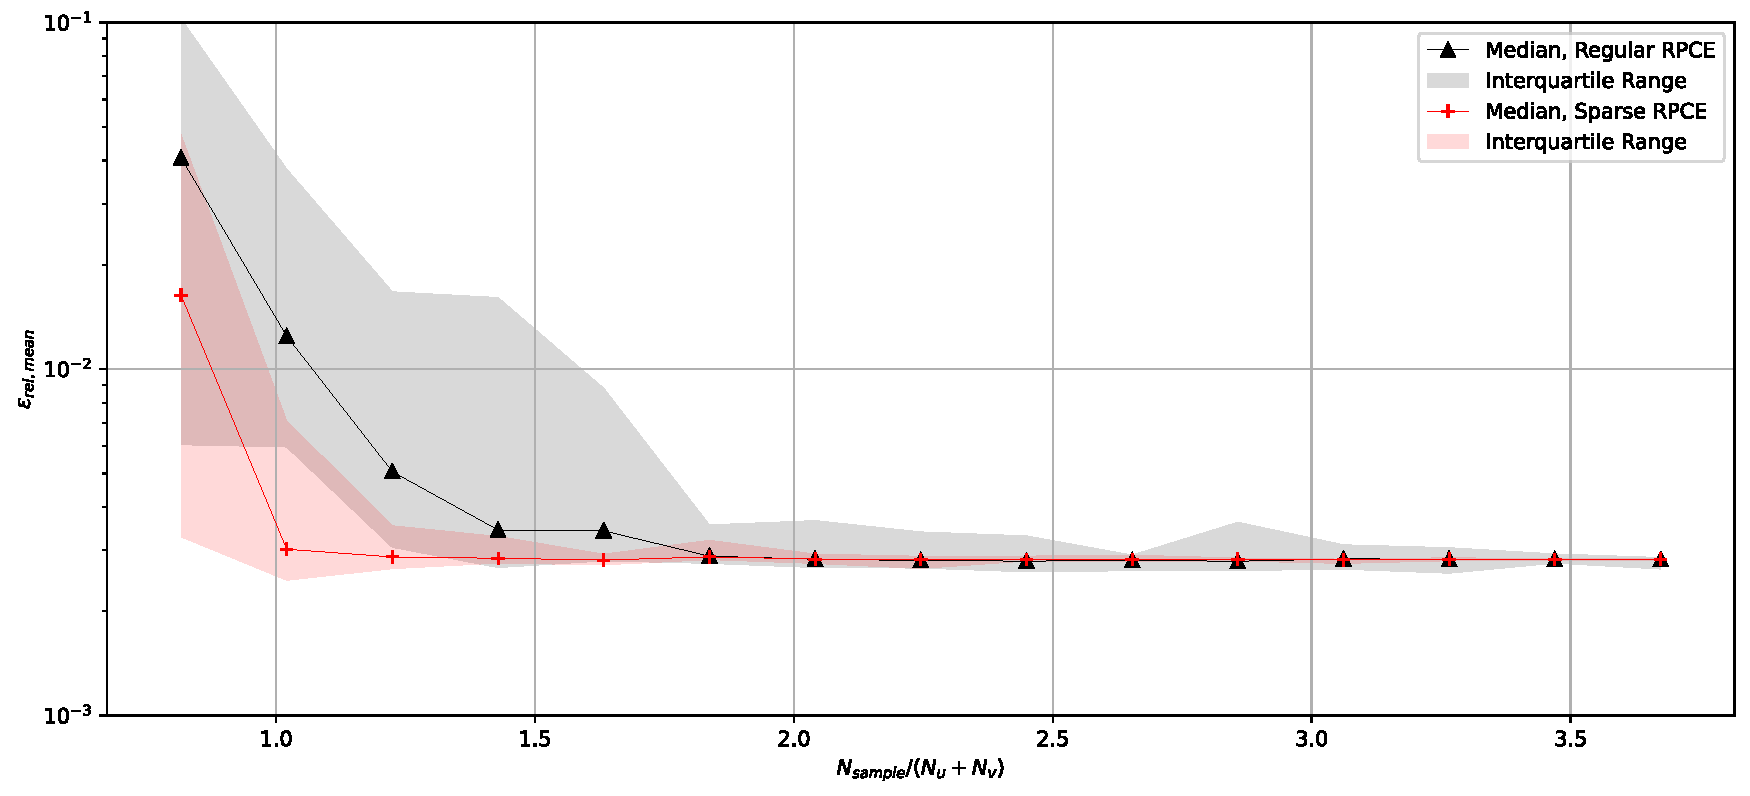
\includegraphics[width=1.0\textwidth]{
        plots/surrogate/plot_2_A_2.pdf
    }
    \caption{%
        Relative Mean Errors of $\left|H_{AA}\right|$ for Regular and Sparse RPCE Models at $\omega=9.0$ rad/s
    }
    \label{mean_sRPCE_A_A_2}
\end{figure}
Figure \ref{var_sRPCE_A_A_2} shows the medians and interquartile ranges of relative variance errors of the FRF approximations for the regular and sparse RPCE models at $\omega=9.0$ rad/s.
\begin{figure}[H]
    \centering
    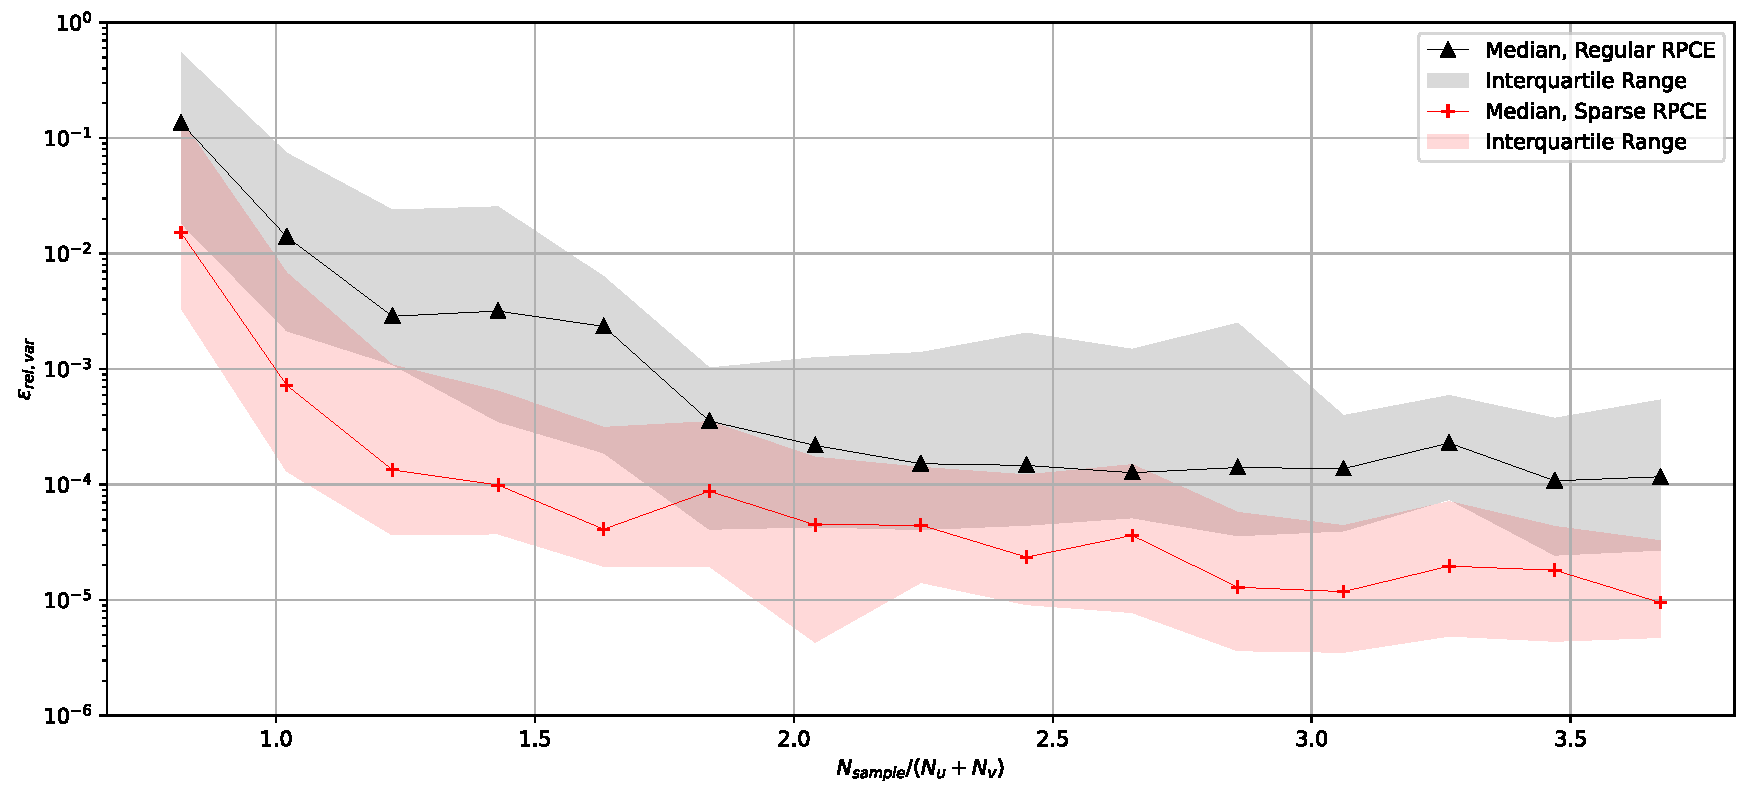
\includegraphics[width=1.0\textwidth]{
        plots/surrogate/plot_3_A_2.pdf
    }
    \caption{%
        Relative Variance Errors of $H_{AA}$ for Regular and Sparse RPCE Models at $\omega=9.0$ rad/s
    }
    \label{var_sRPCE_A_A_2}
\end{figure}
The two figures above show that the sparse RPCE models have lower relative mean errors and relative variance errors when training data sizes are small.
Figures \ref{mean_sRPCE_A_A_3} to \ref{mean_sRPCE_A_A_6} display the relative mean errors of the FRF approximations for regular and sparse RPCE models at various frequencies.
Figures \ref{var_sRPCE_A_A_3} to \ref{var_sRPCE_A_A_6} display the relative variance errors of the FRF approximations for regular and sparse RPCE models at various frequencies.
All figures show similar trends.
% The relative mean errors and relative variance errors at other frequencies are available in the appendix.
\begin{figure}[H]
    \centering
    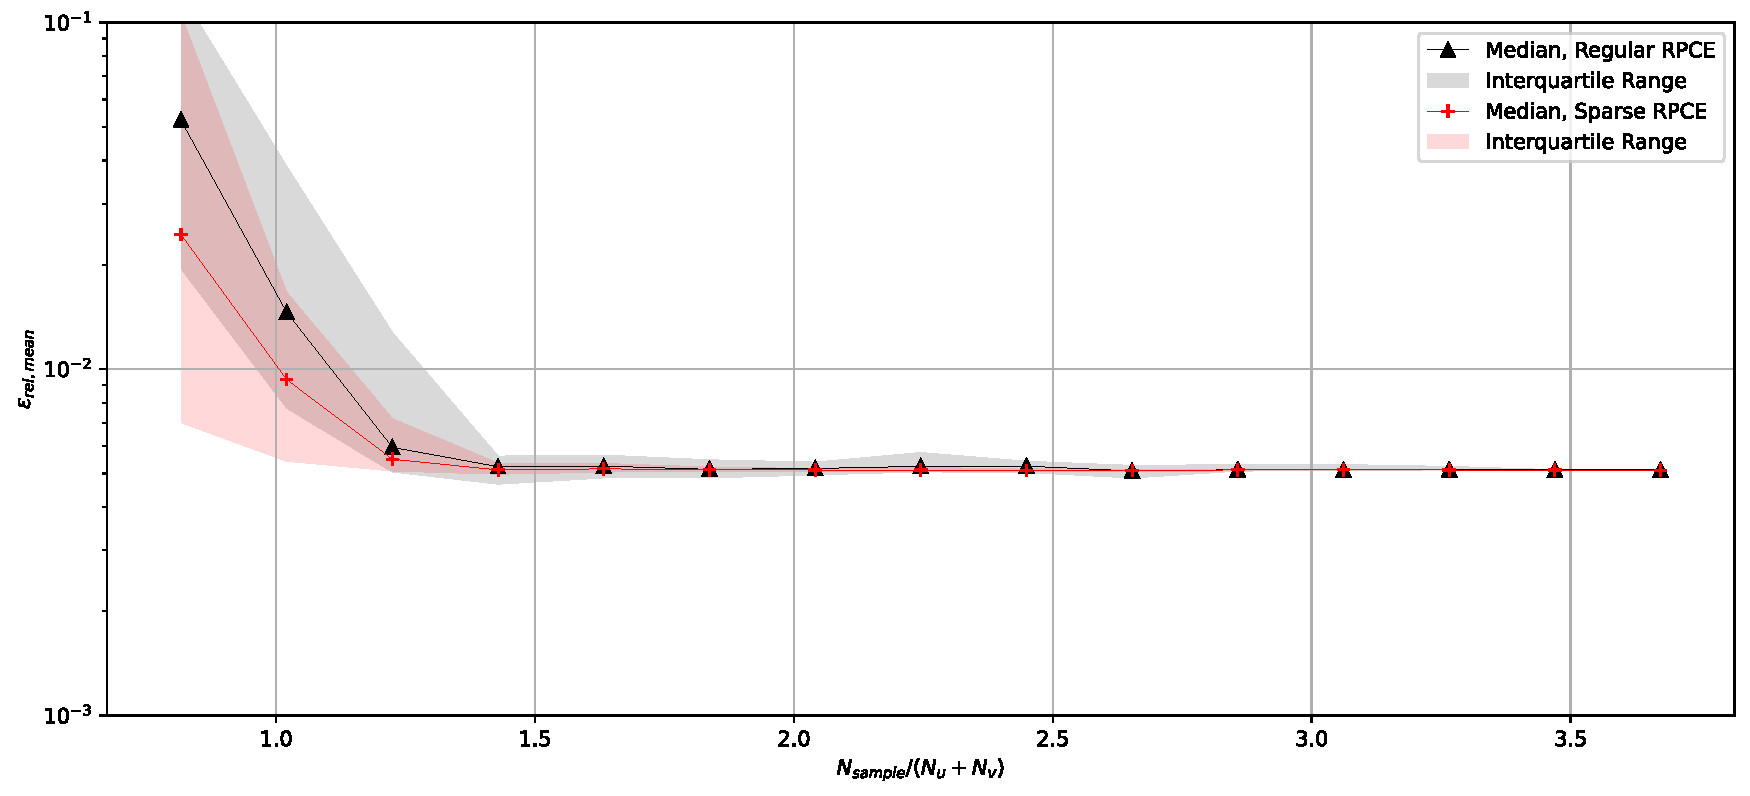
\includegraphics[width=1.0\textwidth]{
        plots/surrogate/plot_2_A_3.pdf
    }
    \caption{%
        Relative Mean Errors of $\left|H_{AA}\right|$ for Regular and Sparse RPCE Models at $\omega=9.5$ rad/s
    }
    \label{mean_sRPCE_A_A_3}
\end{figure}
\begin{figure}[H]
    \centering
    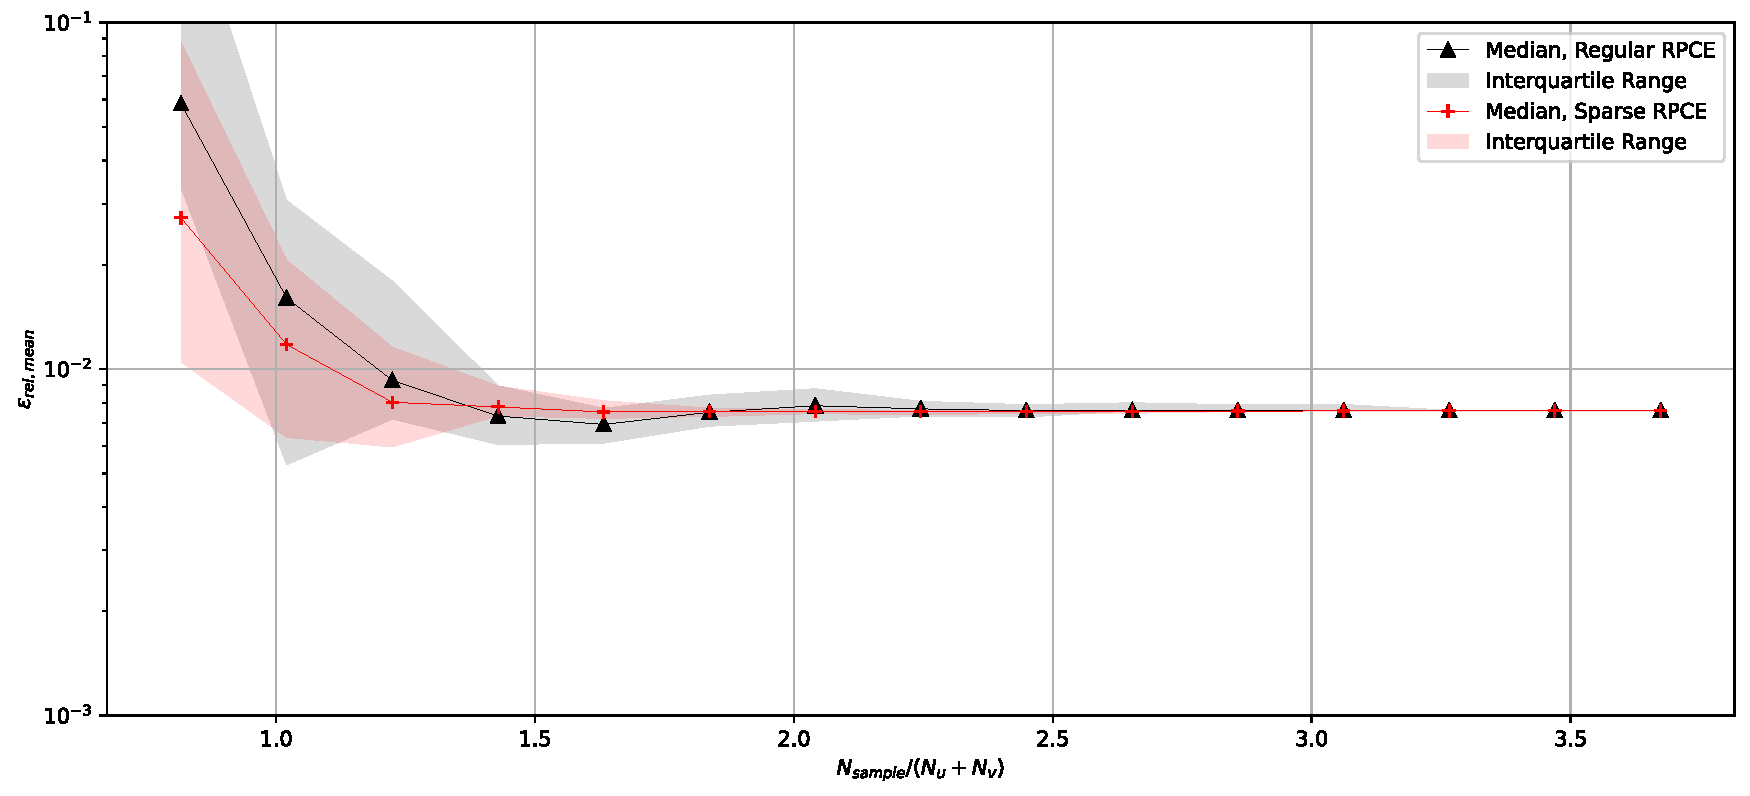
\includegraphics[width=1.0\textwidth]{
        plots/surrogate/plot_2_A_4.pdf
    }
    \caption{%
        Relative Mean Errors of $\left|H_{AA}\right|$ for Regular and Sparse RPCE Models at $\omega=10.0$ rad/s
    }
\end{figure}
\begin{figure}[H]
    \centering
    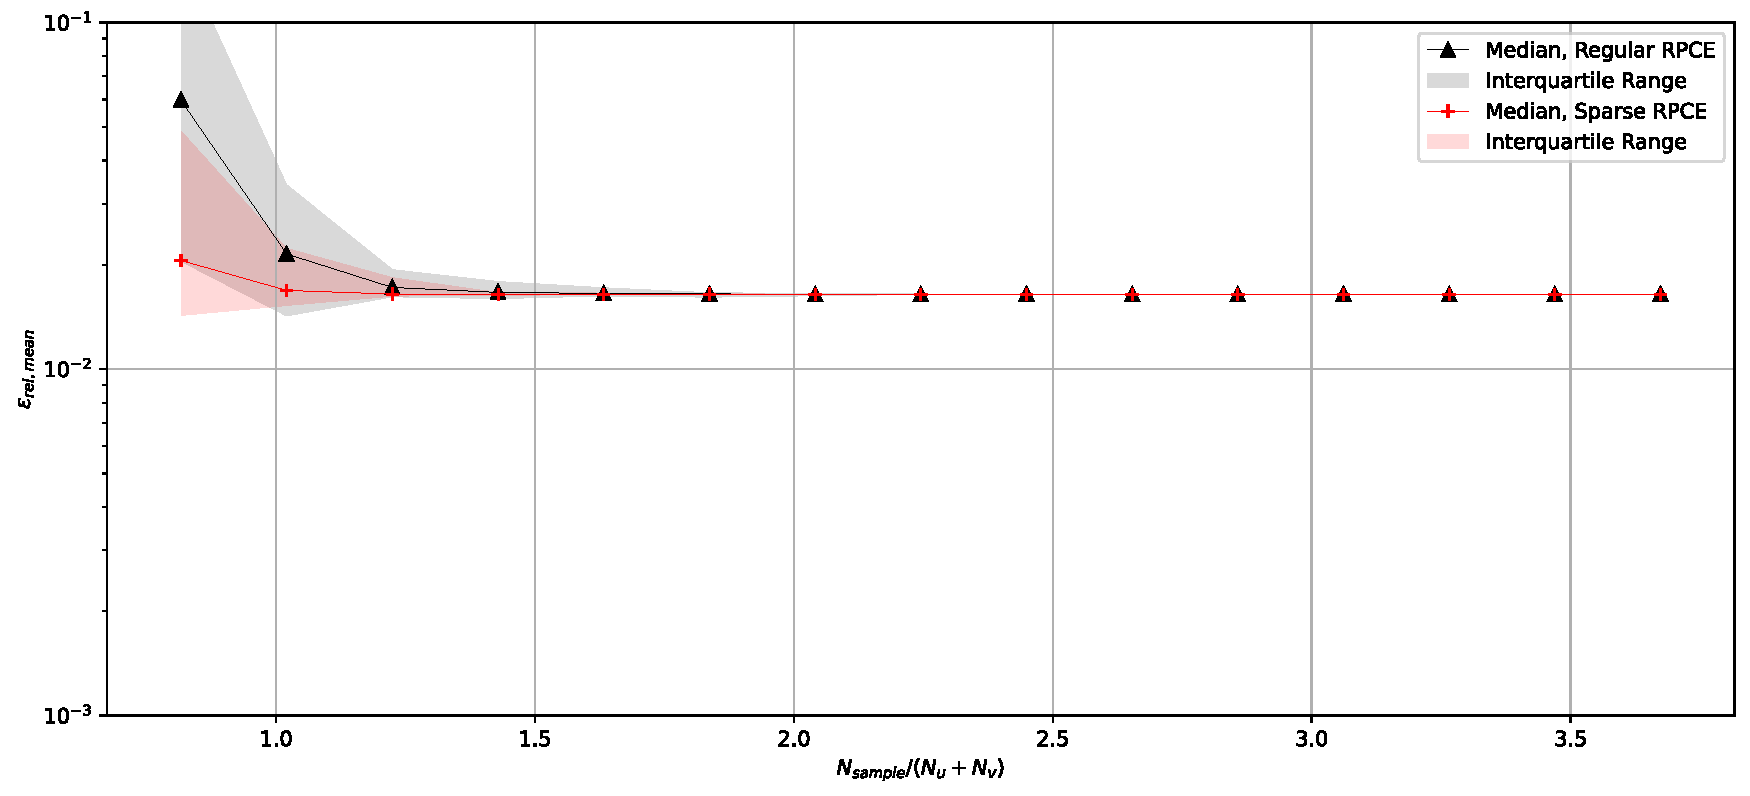
\includegraphics[width=0.85\textwidth]{
        plots/surrogate/plot_2_A_5.pdf
    }
    \caption{%
        Relative Mean Errors of $\left|H_{AA}\right|$ for Regular and Sparse RPCE Models at $\omega=10.5$ rad/s
    }
\end{figure}
\begin{figure}[H]
    \centering
    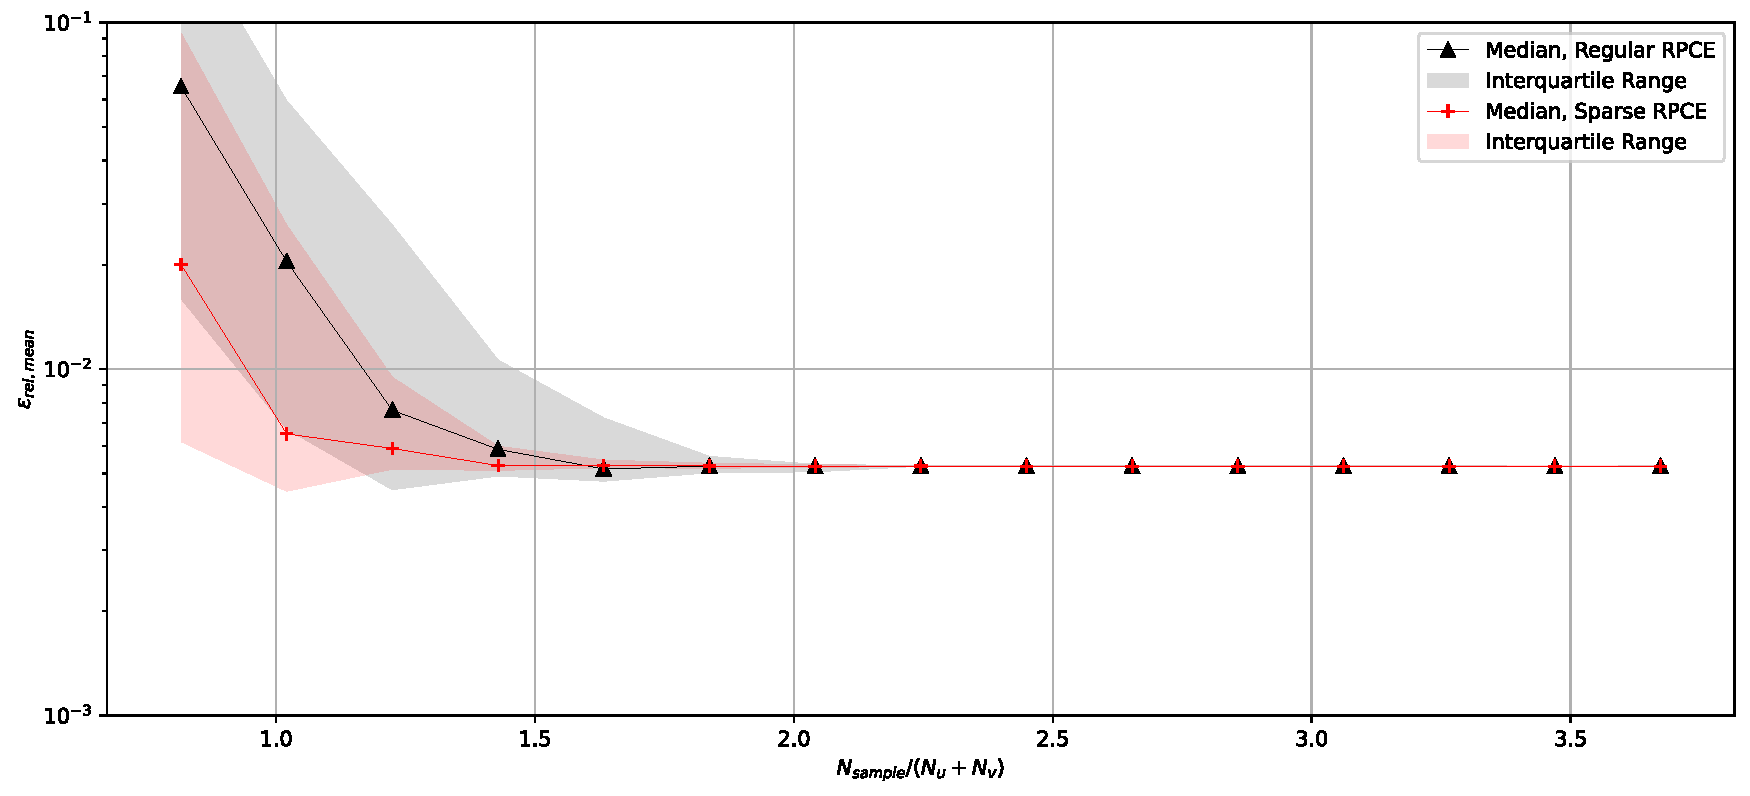
\includegraphics[width=0.85\textwidth]{
        plots/surrogate/plot_2_A_6.pdf
    }
    \caption{%
        Relative Mean Errors of $\left|H_{AA}\right|$ for Regular and Sparse RPCE Models at $\omega=11.0$ rad/s
    }
    \label{mean_sRPCE_A_A_6}
\end{figure}
\begin{figure}[H]
    \centering
    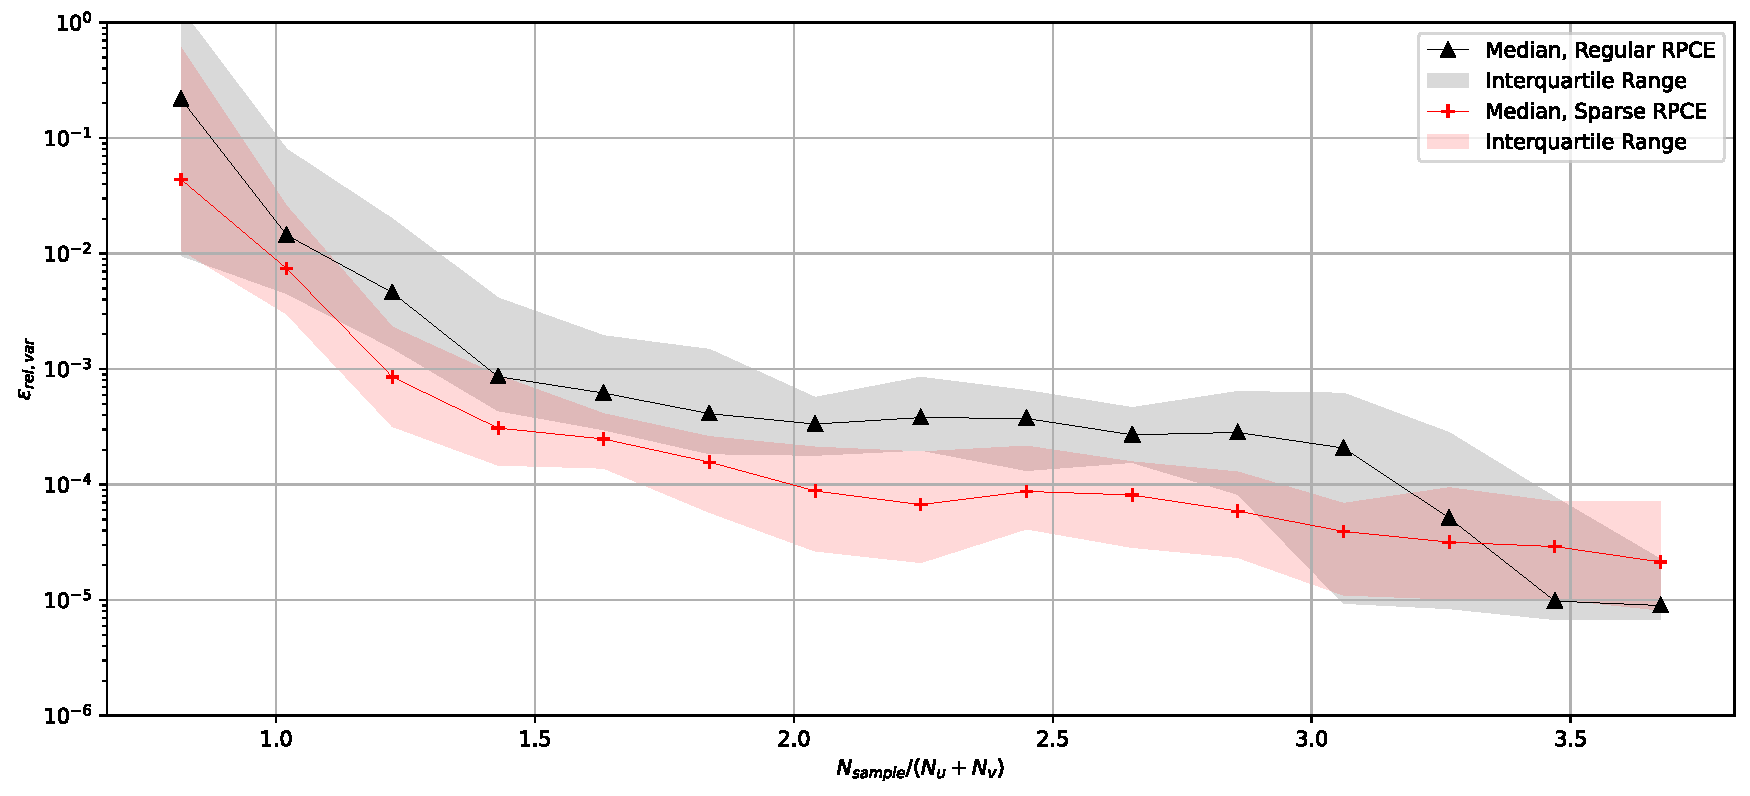
\includegraphics[width=0.85\textwidth]{
        plots/surrogate/plot_3_A_3.pdf
    }
    \caption{%
        Relative Variance Errors of $H_{AA}$ for Regular and Sparse RPCE Models at $\omega=9.5$ rad/s
    }
    \label{var_sRPCE_A_A_3}
\end{figure}
\begin{figure}[H]
    \centering
    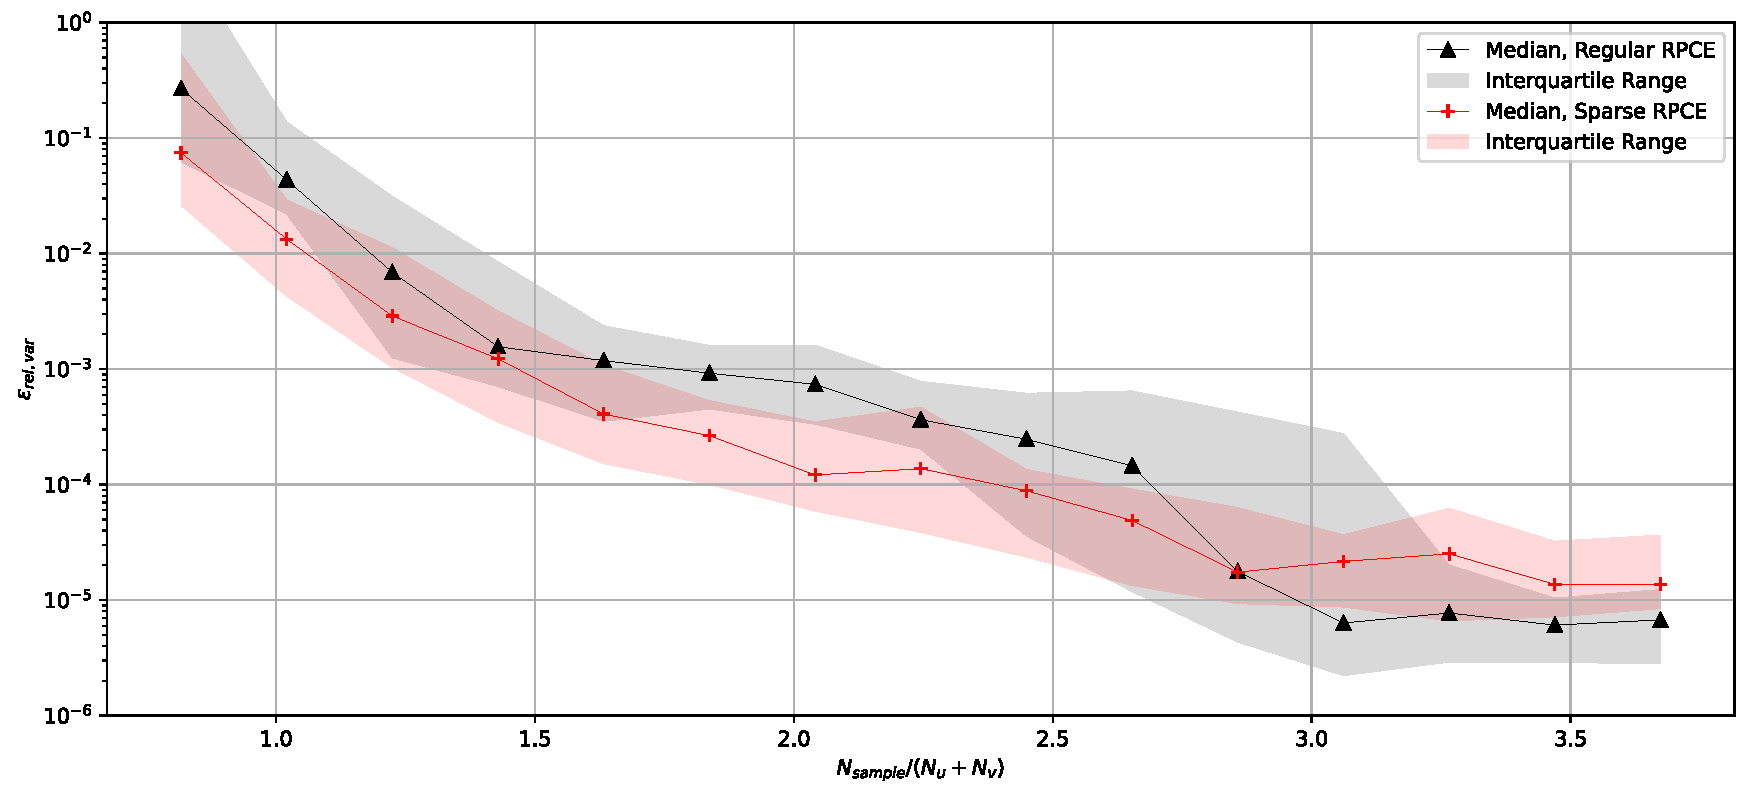
\includegraphics[width=0.85\textwidth]{
        plots/surrogate/plot_3_A_4.pdf
    }
    \caption{%
        Relative Variance Errors of $H_{AA}$ for Regular and Sparse RPCE Models at $\omega=10.0$ rad/s
    }
\end{figure}
\begin{figure}[H]
    \centering
    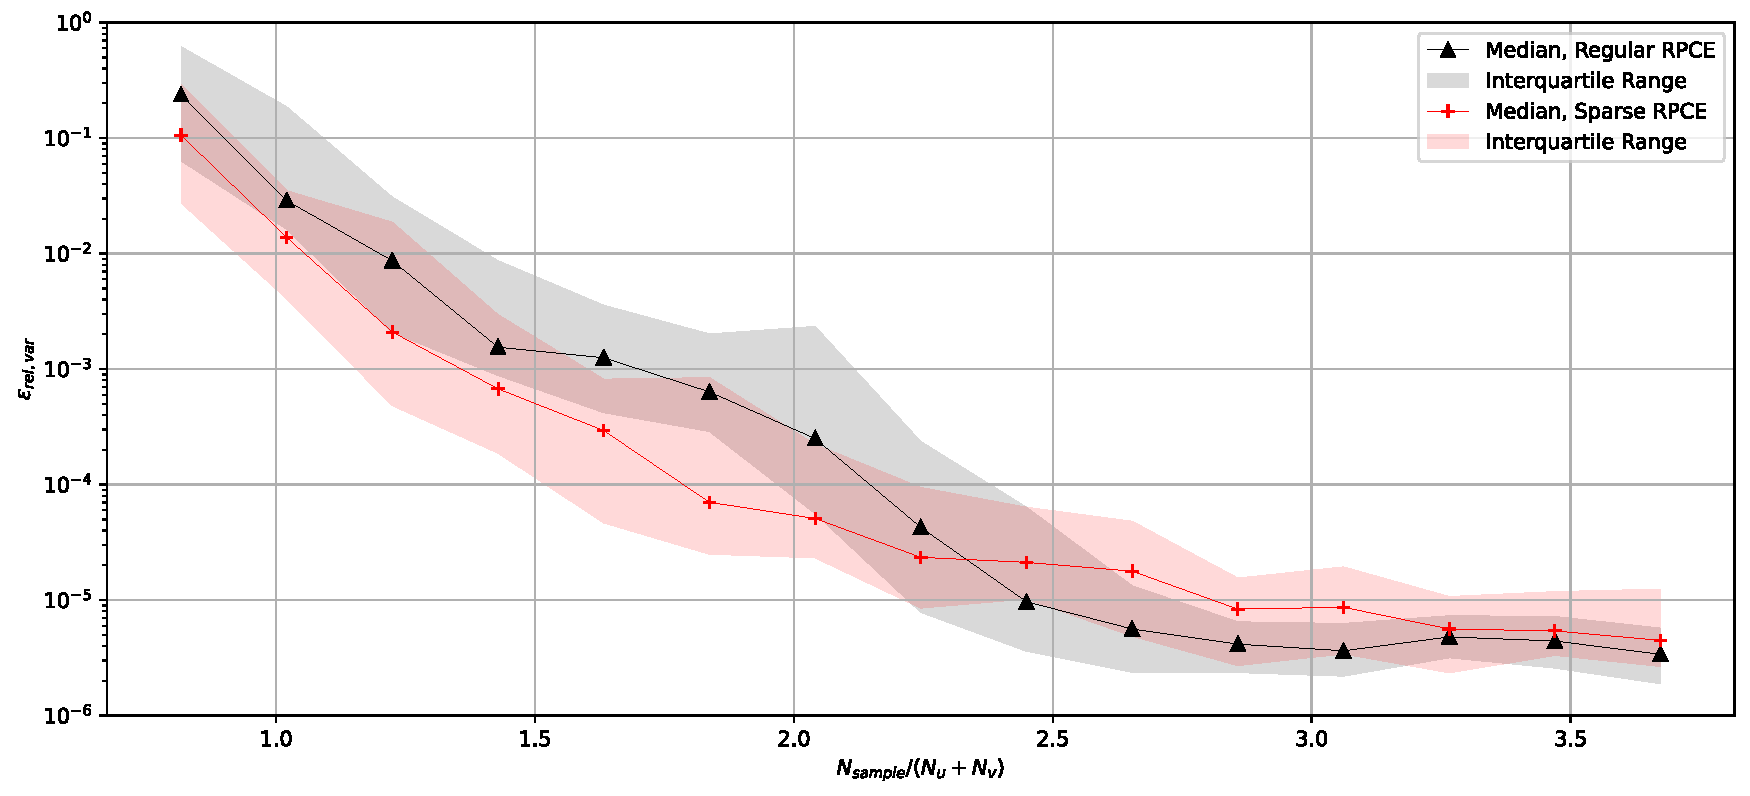
\includegraphics[width=0.85\textwidth]{
        plots/surrogate/plot_3_A_5.pdf
    }
    \caption{%
        Relative Variance Errors of $H_{AA}$ for Regular and Sparse RPCE Models at $\omega=10.5$ rad/s
    }
\end{figure}
\begin{figure}[H]
    \centering
    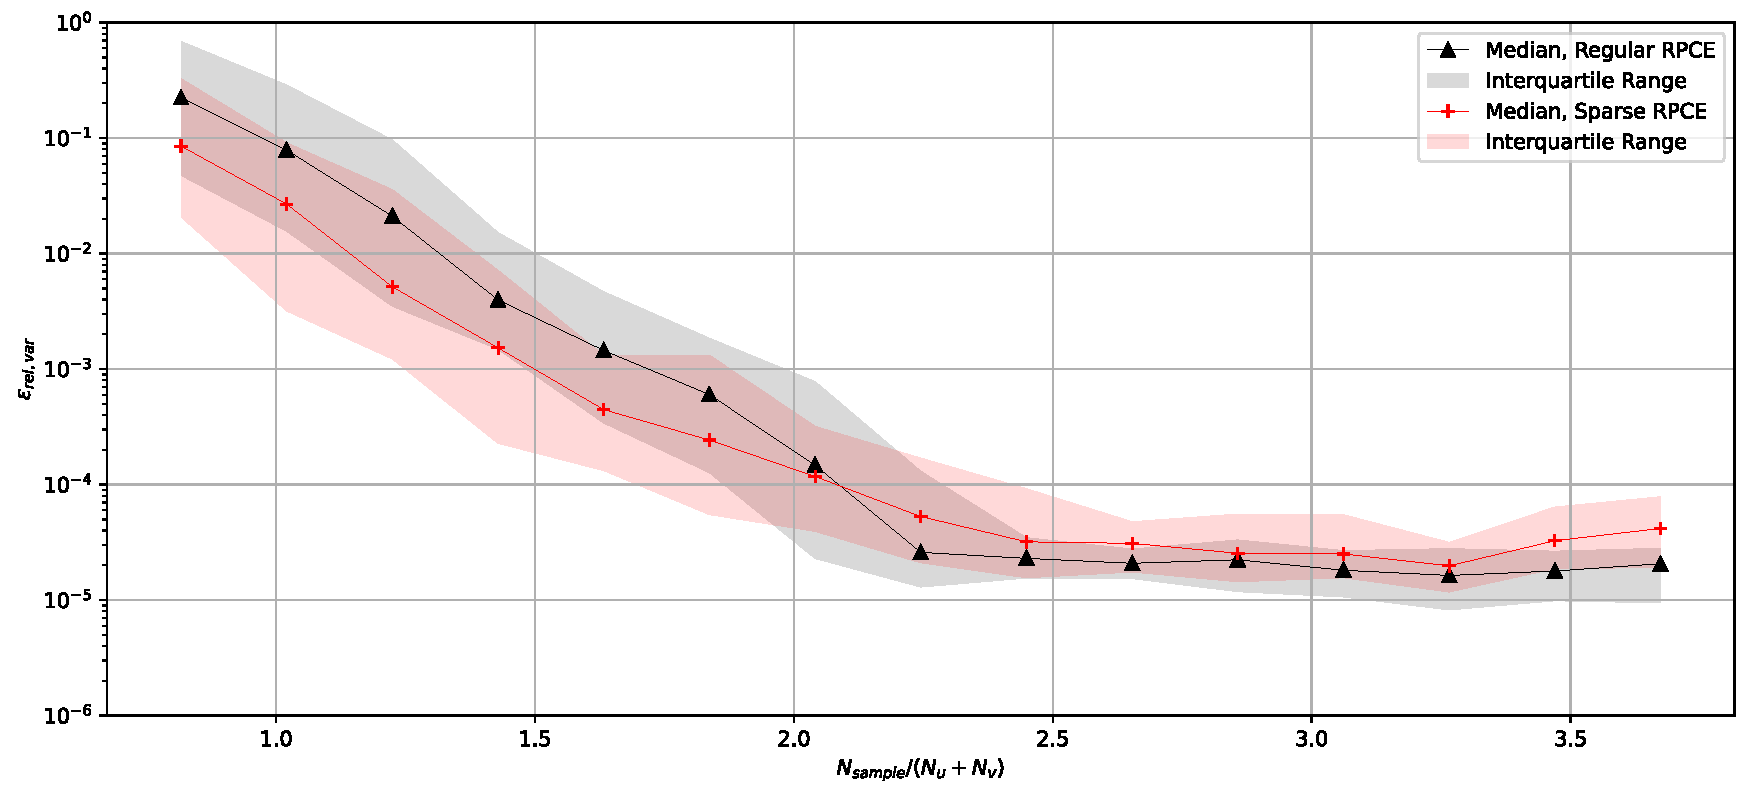
\includegraphics[width=0.85\textwidth]{
        plots/surrogate/plot_3_A_6.pdf
    }
    \caption{%
        Relative Variance Errors of $H_{AA}$ for Regular and Sparse RPCE Models at $\omega=11.0$ rad/s
    }
    \label{var_sRPCE_A_A_6}
\end{figure}